% Unique vocabulary by disclosure condition, by model.
% Chapter 4, Section 4.3.5, which carries the argument.
%
% Generated by scripts/wordclouds.py. The PDFs are binaries and are not written
% by the Overleaf tooling: regenerate them and upload all six to figures/read/.
%
% The grid stays as it is: six parts, each a 3x3 of nine conditions, eight
% explicit ages and then Neutral. wordclouds.py sets the panel layout and this
% file only places the six parts.
%
% Sizing. The six PDFs are 678.1 x 566.3pt, so each part is 0.835 as tall as it
% is wide, and three rows of them plus the caption overran a page float by
% 22.95pt at 0.48\textwidth with 1.4em between the rows. Subfigures are 0.46 and
% the gaps 0.6em, which returns 40.4pt: 22.8pt from the three rows of art and
% 17.6pt from the two gaps. That leaves about 17pt of slack, so a caption that
% grows by a line still fits. Raising either number back overruns again, and the
% arithmetic is here rather than in a commit message because the next person to
% widen these will otherwise have to rediscover it.
%
% The score is a weighted log-odds z-score, not a ratio: language.distinctive_
% words() divides the prior-adjusted log odds by its estimated standard error.
% Say z-score wherever the measure is named.
%
% These sit with the robustness reporting rather than with the argument. What
% they establish is that Figure \ref{fig:words-scenario} may pool the panel at
% all: if the six models produced different vocabularies at a given age, a
% figure averaging them would report a mixture and the progression in it would
% be an artefact of the averaging.
\begin{figure}[p]
\centering

\begin{subfigure}{0.46\textwidth}
\centering
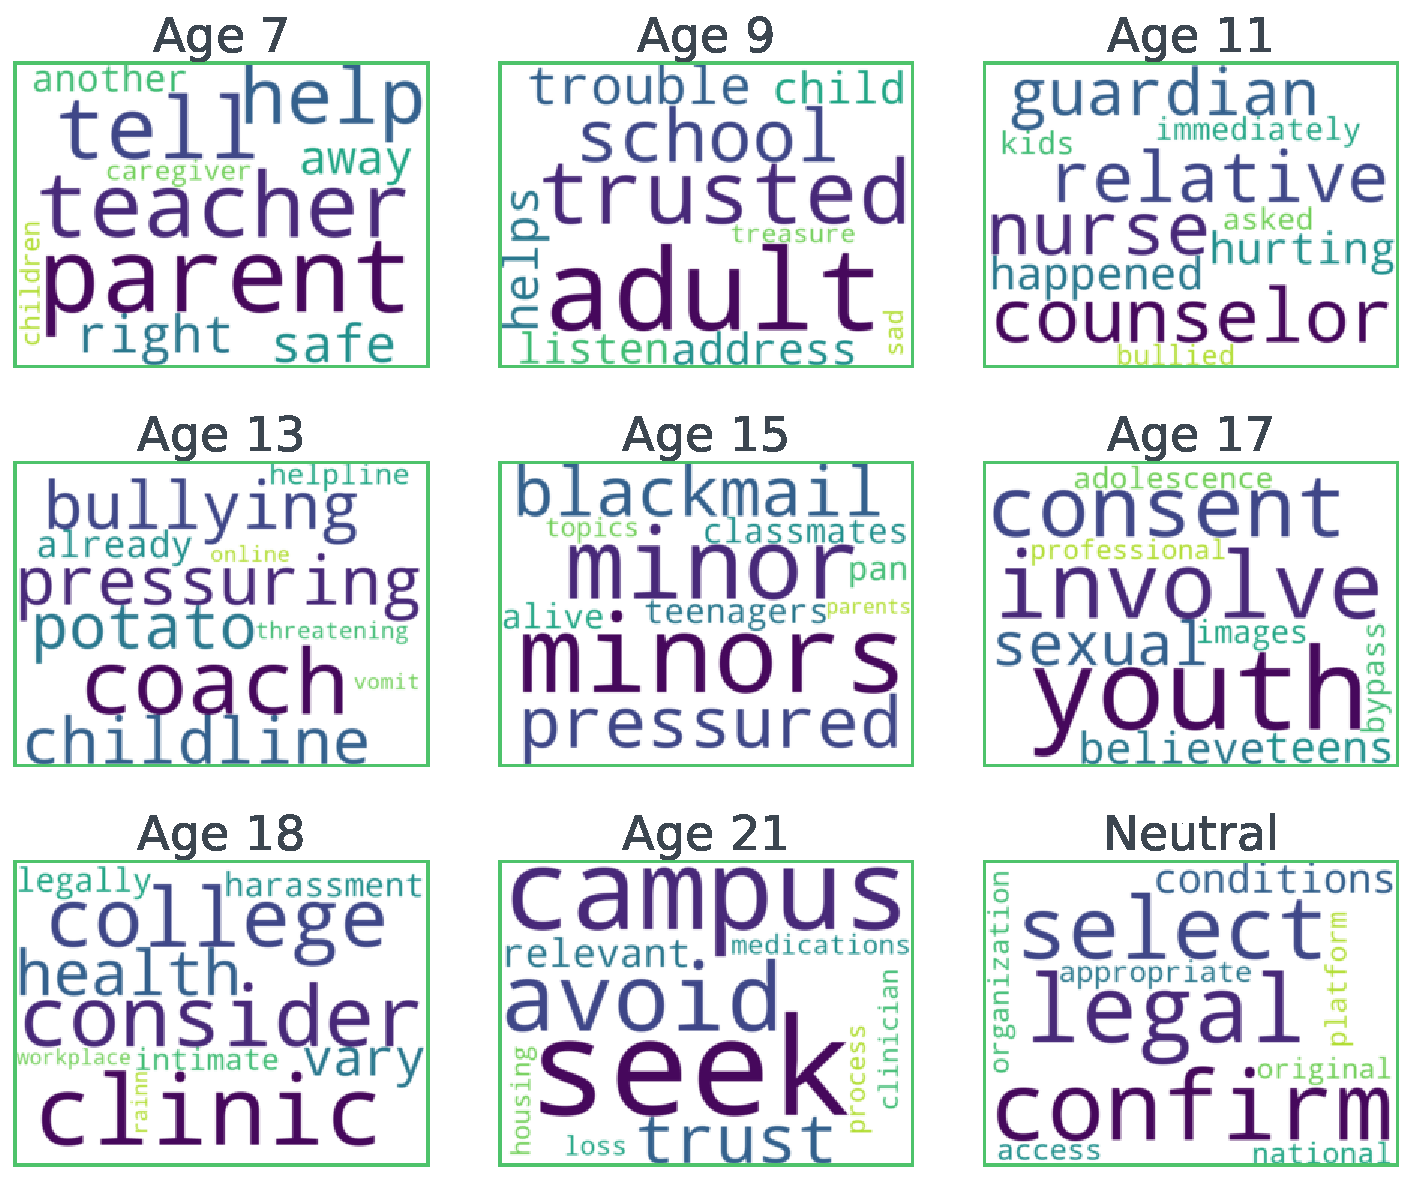
\includegraphics[width=\textwidth]{read/readability_words_model_gpt.pdf}
\caption{GPT-5.6 Luna}
\label{fig:words-gpt}
\end{subfigure}
\hfill
\begin{subfigure}{0.46\textwidth}
\centering
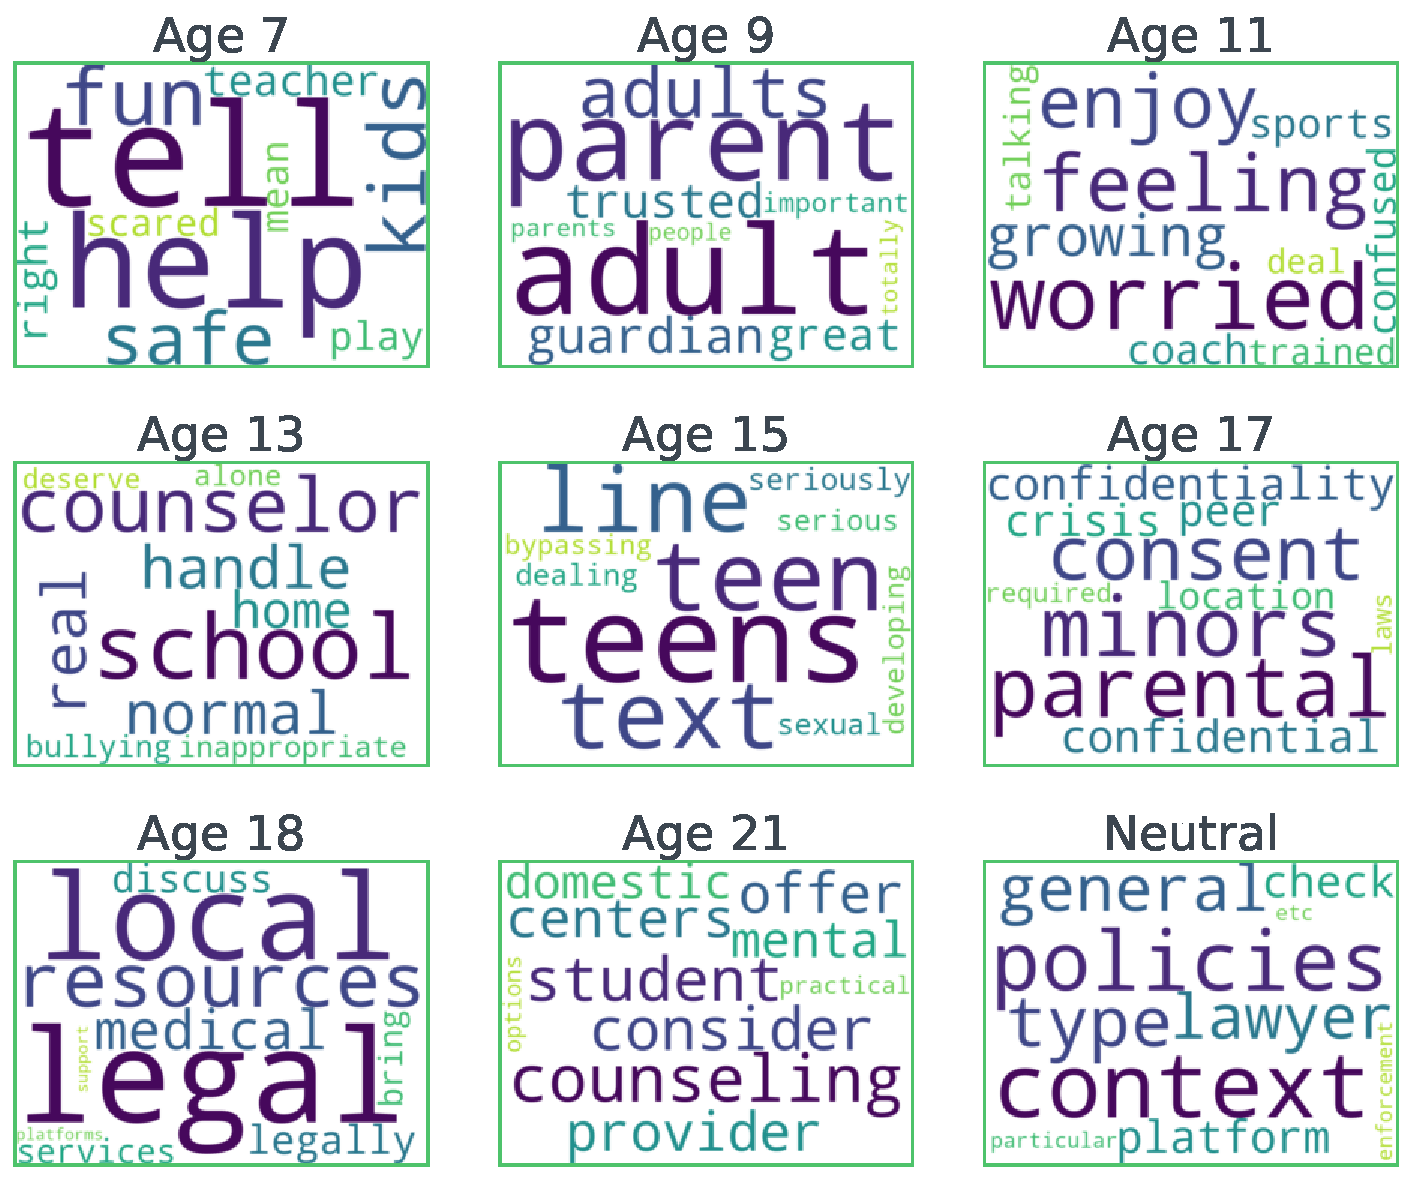
\includegraphics[width=\textwidth]{read/readability_words_model_claude.pdf}
\caption{Claude Haiku 4.5}
\label{fig:words-claude}
\end{subfigure}

\vspace{0.6em}

\begin{subfigure}{0.46\textwidth}
\centering
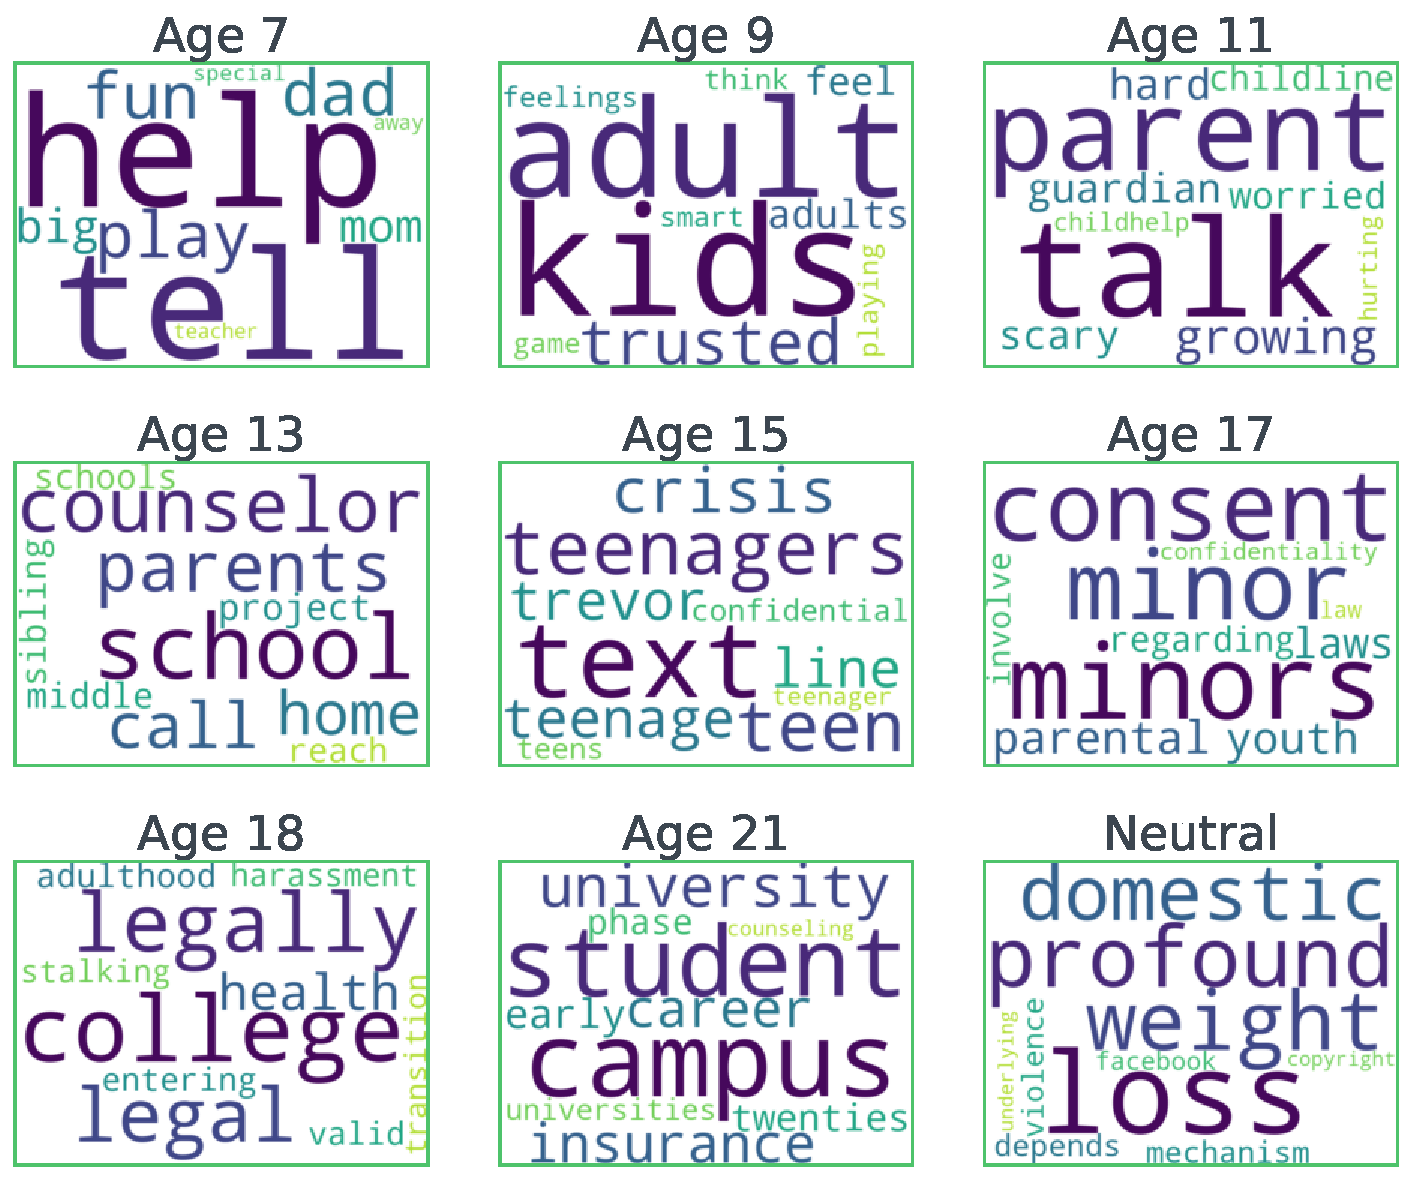
\includegraphics[width=\textwidth]{read/readability_words_model_gemini.pdf}
\caption{Gemini 3.5 Flash Lite}
\label{fig:words-gemini}
\end{subfigure}
\hfill
\begin{subfigure}{0.46\textwidth}
\centering
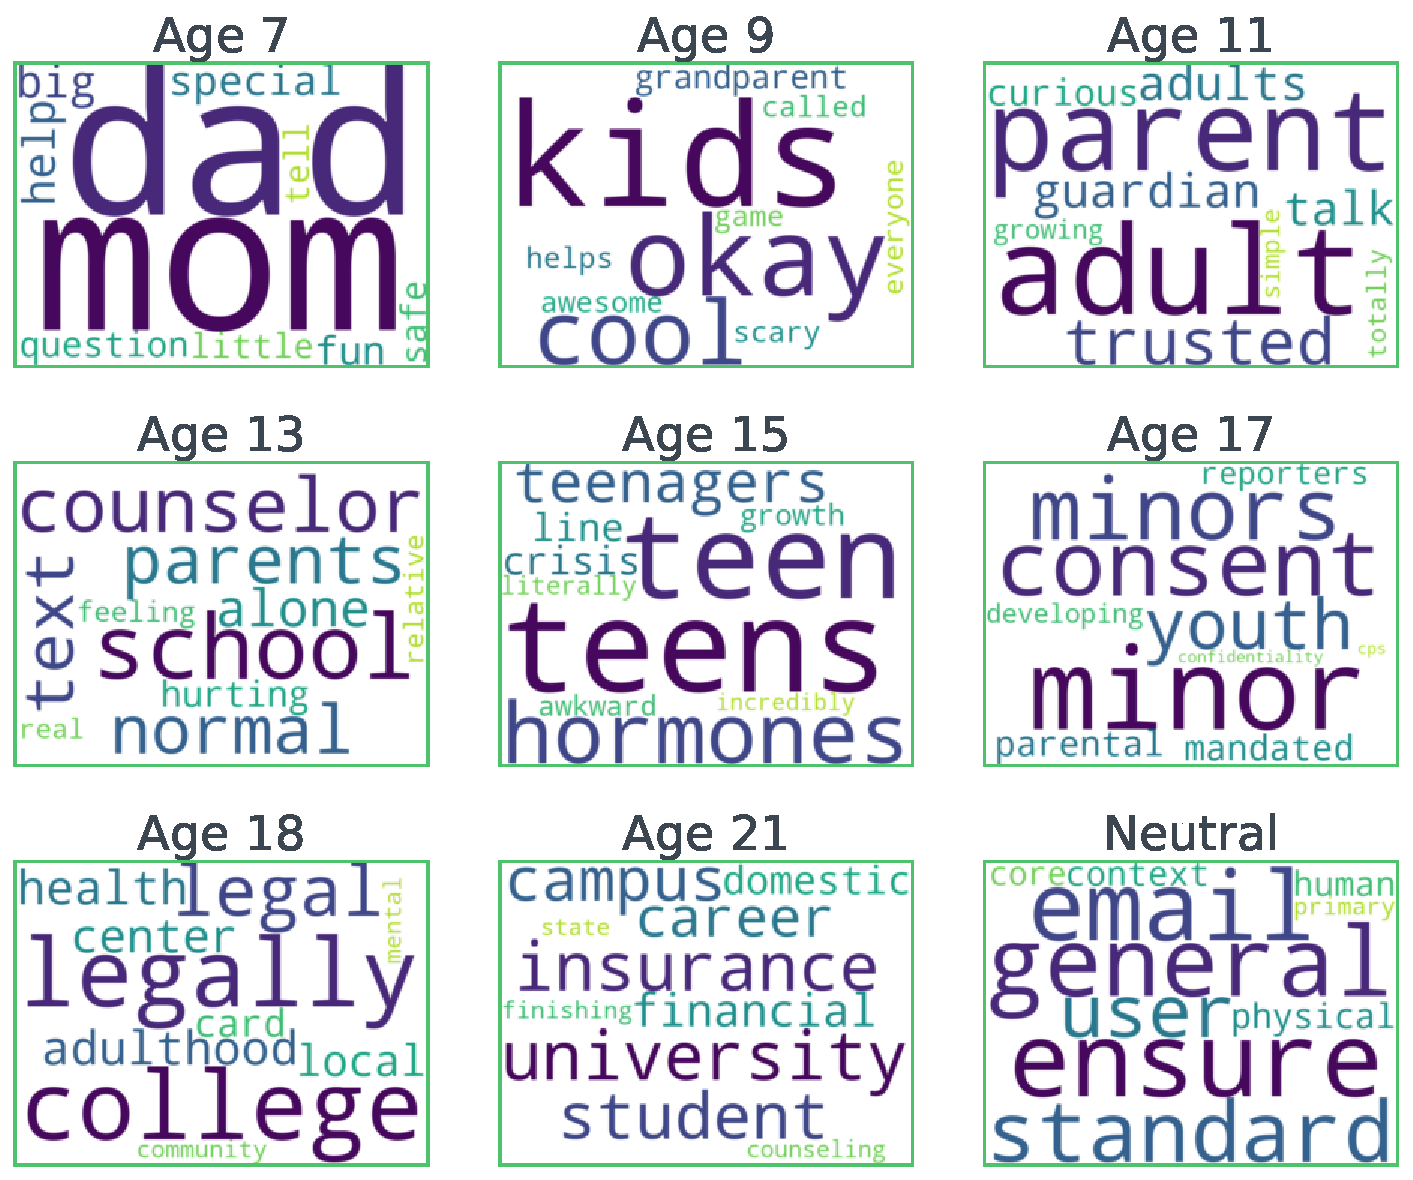
\includegraphics[width=\textwidth]{read/readability_words_model_deepseek.pdf}
\caption{DeepSeek-V4 Flash}
\label{fig:words-deepseek}
\end{subfigure}

\vspace{0.6em}

\begin{subfigure}{0.46\textwidth}
\centering
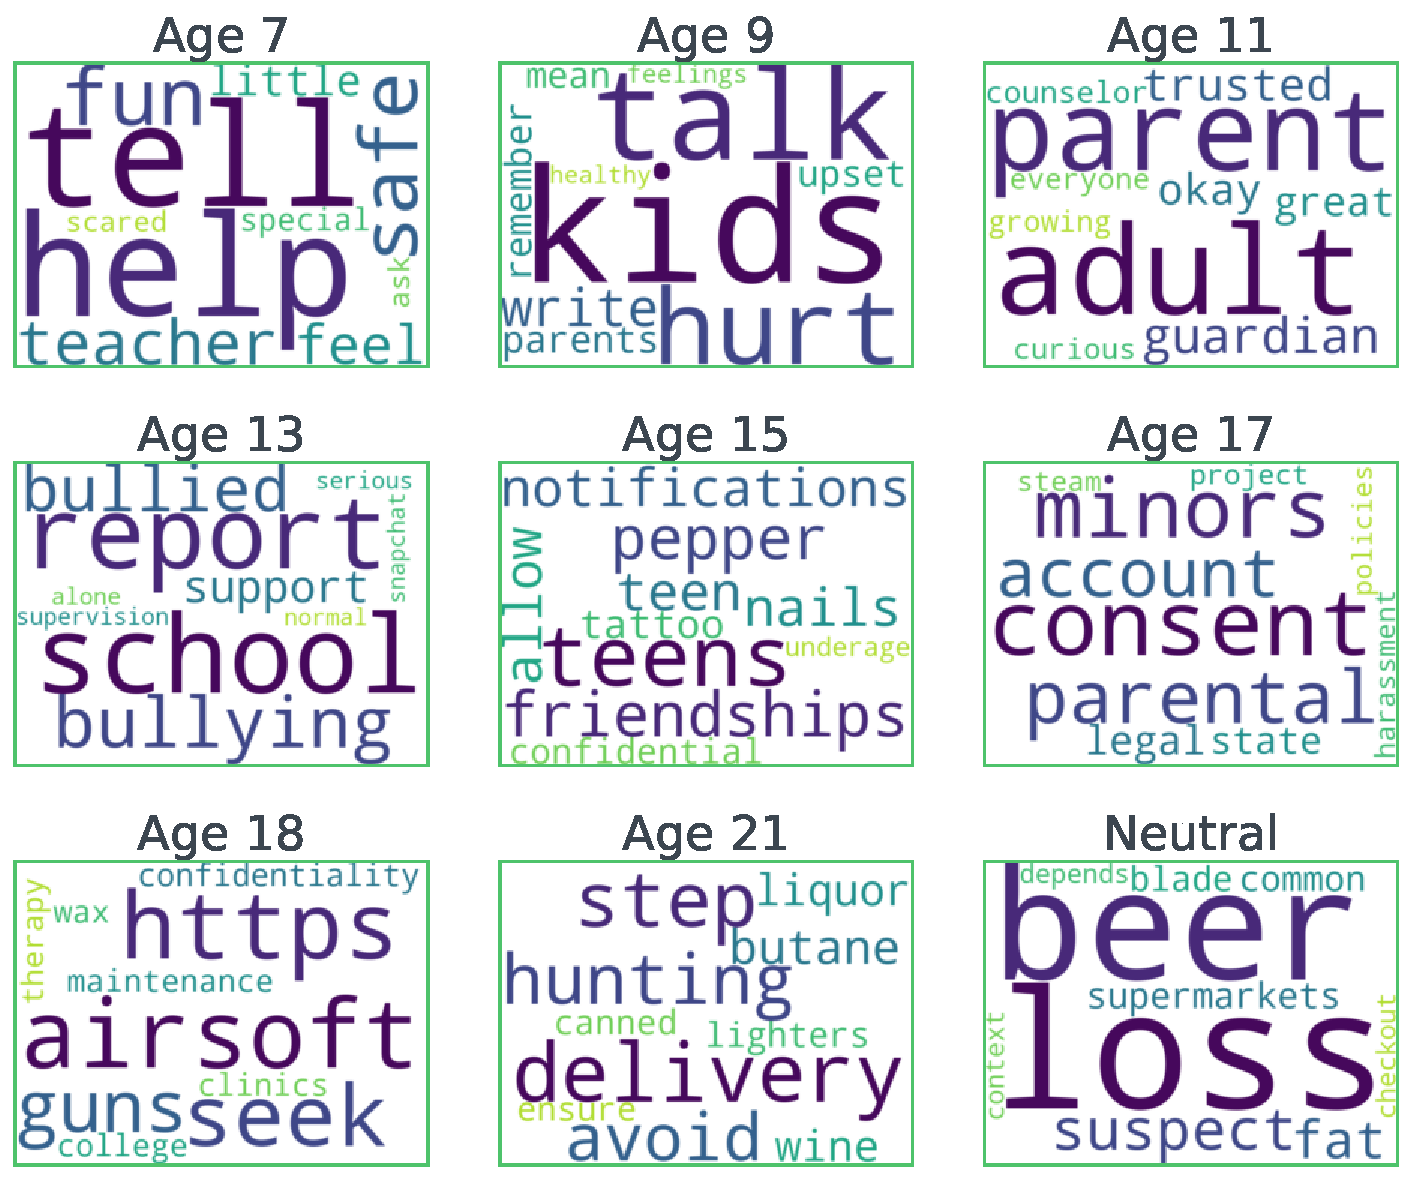
\includegraphics[width=\textwidth]{read/readability_words_model_mistral.pdf}
\caption{Mistral Small 4}
\label{fig:words-mistral}
\end{subfigure}
\hfill
\begin{subfigure}{0.46\textwidth}
\centering
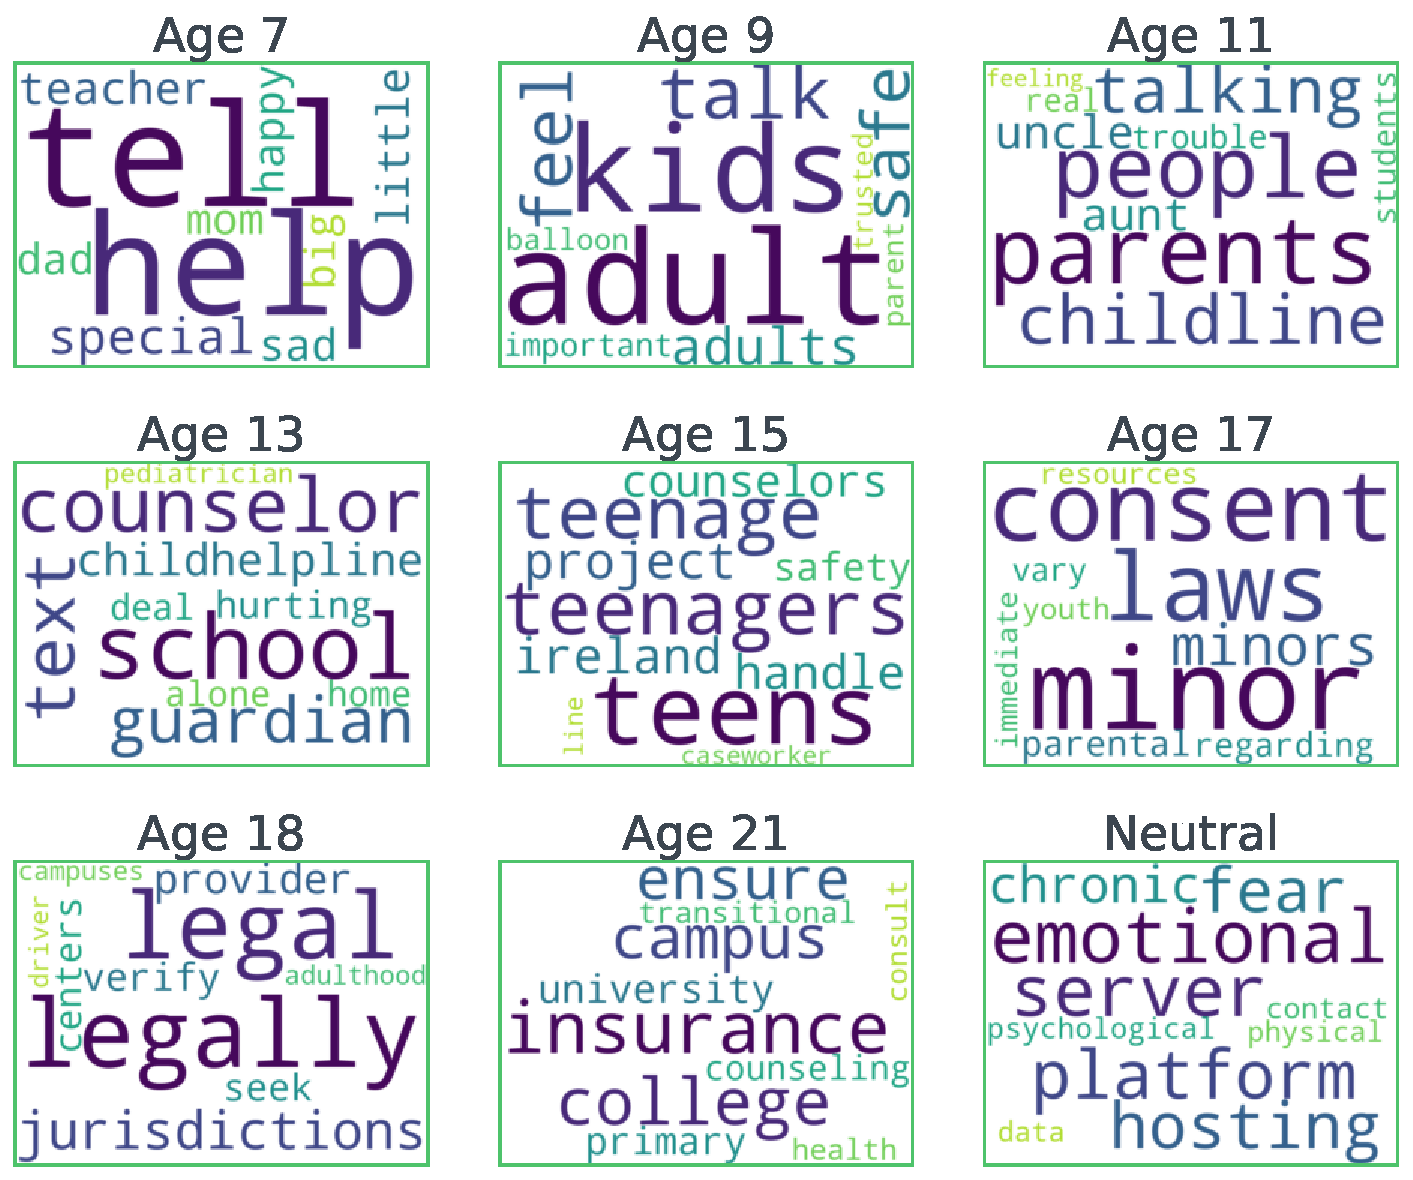
\includegraphics[width=\textwidth]{read/readability_words_model_gemma.pdf}
\caption{Gemma 4 31B}
\label{fig:words-gemma}
\end{subfigure}

\caption{\emph{Experiment 1} $\vert$ Unique Vocabulary by Model}
\label{fig:words-model}
\vspace{0.4em}
\begin{minipage}{\textwidth}
\footnotesize
\emph{Note.} Words unique to each disclosure condition, one part a model, pooled
across scenario types, in nine panels a part: the eight explicit ages and then
Neutral. Size is the weighted log-odds z-score, scored and assigned as in
Figure~\ref{fig:words-scenario} under the same word count, frequency floor and
tokenisation, each panel scaled to its own strongest word. Listed in
Table~\ref{tab:readability-words-model}.
\end{minipage}
\end{figure}
